\documentclass[12pt]{article} 
\usepackage{url,graphicx,tabularx,array}
\usepackage[margin=.5in,nohead,nofoot]{geometry} 
\usepackage{color}

\begin{document} 

\title{The EPOCH Particle in Cell simulation codes}
\author{C.S.Brady}
\maketitle
\tableofcontents
\newpage

\section{FAQs}
\subsection{What is EPOCH?}
Epoch is a plasma physics simulation code which uses the Particle in Cell(PIC) method. In this method, collections of physical particles are represented using a smaller number of pseudoparticles, and the fields generated by the motion of these pseudoparticles are calculated using a finite difference time domain technique on an underlying grid of fixed spatial resolution. The forces on the pseduoparticles due to the calculated fields are then used to update the pseudoparticle velocities, and these velocities are then used to update the pseudoparticle positions. This leads to a scheme which can reproduce the full range of classical microscale behaviour of a collection of charged particles, but shows statistical noise if one pseudoparticle represents many real particles (which is common in real problems), and also shows artificial smoothing of currents and fields due to the finite spatial resolution of the underlying grid.\\
This approach can alternatively be considered as using the pseduoparticles as Monte Carlo sampling points of the full (2N)D phase space of an (N)D problem. This has siginifcant memory advantages of (2N)D direct Vlasov solvers at the expense of lower accuracy and higher noise.
\subsubsection{Features of EPOCH}
\begin{itemize}
\item MPI parallelised explicit 2nd order relativistic PIC code
\item Dynamic MPI load balancing option
\item MPIIO based output, allowing restart on arbitrary number of processors
\item Data analysis and visualisation options include ITT IDL, LLNL VisIT and Mathworks MatLab
\end{itemize}
\subsection{The origins of the code}
The EPOCH family of PIC codes is based on the older code PSC by Hartmut Ruhl, and retains almost the same core algorithm for the field updates and particle advance routines. EPOCH was written to add more modern features, and to structure the code in such a way that future expansion of the code is made as easy as possible.
\subsection{What normalisations are used in EPOCH?}
Since the idea from the start was that EPOCH would be used by a large number of different users, and that it should be as easy as possible to ``plug in'' different modules from different people into a given copy of the code, it was decided to write EPOCH in SI units. There are a few places in the code where some quantities are given in other units for convenience(for example charges are specified in multiples of the electron charge), but the entire of the core code is written in SI units.
\subsection{What are those \_num things doing everywhere}
Historically using the compiler autopromotion of REAL to DOUBLE PRECISION was unreliable, so EPOCH uses kind tags to specifiy the precision of the code. The \_num suffixes and the associated definition of REALs as REAL(num) are these kind tags in operation. The \_num tags force numerical constants to match the precision of the code preventing errors due to precision conversion. The important thing is that all numerical constants should be tagged with an \_num tag, and all REALs should be defined as REAL(num).
\subsection{I just want to use the code as a black box, or I'm just starting. How do I do that?}
See the section titled {\bf EPOCH for end users}
\subsection{I can set up the code using the autoloaders, but I want more control. How do I do that?}
See the section titled {\bf EPOCH for advanced end users}
\subsection{I want to add additional output variables from the code. How do I do that?}
See the section titled {\bf EPOCH data output}
\subsection{I want to add additional physics to the code. How do I do that?}
See the section titled {\bf Expanding EPOCH}
\subsection{I am an advanced user, but I want to set up the code so that less experienced users can use it. How do I do that?}
See the section titled{\bf Customising EPOCH}
\subsection{I want to have a full understanding of how EPOCH works. How do I do that?}
You're insane. Seek professional help.

\section{EPOCH for end users}
\subsection{Structure of the EPOCH codes}
When obtained, the EPOCH codes all have a similar structure. Inside the epoch{n}d directory, there are 4 subdirectories
\begin{itemize}
\item src - The EPOCH source code
\item IDL - The IDL routines needed to open the Compact Flexible Datatype (CFD) files which the code outputs
\item VisIT - The files for creating a plugin for the LLNL VisIT parallel visualisation tool for reading CFD files
\item Data - A sample data directory containing example input deck files
\end{itemize}
there are also 8 files
\begin{itemize}
\item cleandir - A script which deletes the output files generated by the EPOCH code from an output directory while leaving the input files needed to run the code
\item copydir - A script which copies the input files used by EPOCH from one directory to another without copying any of the output files
\item deck.file - An example file showing how to run the code without user interaction. It will be explained in more depth later
\item epoch.pbs - An example PBS batch submission script showing how to use the code in a parallel environment. In general, it probably will not be suitable for your particular machine, please consult the documentation for the facility that you are working on.
\item Makefile - A standard makefile
\item pack\_for\_transport - A script which is used in the event of bug reporting. pack\_for\_transport packs up all the relevant parts of a standard EPOCH installation into a single tgz file. The file is then sent when reporting the bug.
\item Start.pro - An IDL script which starts the IDL visualisation routines. Execute it using ``idl Start''
\end{itemize}

\subsection{Libraries and requirements}
The EPOCH codes are written using MPI for parallelism, but have no other libraries or dependencies. Currently, the codes are written to only require and MPI1.2 compatible compiler, although this may change to require full MPI2 compliance in the future. Current versions of both MPICH and OpenMPI are full MPI2 implementations and are known to work with this code. The SCALI MPI implementation is only a full MPI1.2 implementation and may loose support soon.\\

It is not possible to rewrite the code to remove the dependancy on the MPI libraries without a massive rewrite, which there are no plans to perform.

\subsection{Compiling and running EPOCH}

To compile EPOCH in the supplied state, just type\\
\texttt{make}\\
and the code will compile. There are certain options within the code which are controlled by compiler pre-processors which are described in the next section. When the code is compiled, it creates a new directory called ``bin'' which contains the compiled binary which will be called \texttt{epoch1d}, \texttt{epoch2d} or \texttt{epoch3d}. To run the code, just execute the binary file by typing\\
\texttt{./bin/epoch2d}\\
or whatever the correct binary is for the dimensionality of the code that you have. You should be given a screen which begins with the EPOCH logo, and then reads\\

\begin{verbatim}

Welcome to EPOCH2D Version 1.2

 Specify output directory

\end{verbatim}

At this point, the user simply types in the name of the (already existing) output directory and the code will read the input deck files inside the specified directory and start running. To run the code in parallel, just use the normal mpirun or mpiexec scripts supplied by your MPI implementation. If you want the code to run unattended, then you will need to specify the output directory by piping the directory name in from a file. An example of such a file is supplied as ``deck.file'' with the standard distribution of EPOCH. To use it, just run the code as\\
\texttt{mpirun -np 2 ./bin/epoch2d < deck.file}\\
and the code will run without user input. Some cluster queuing systems do not allow the use of input pipes to mpirun. In this case, there is usually a ``-stdin'' command line option to specify an input file, see your cluster documentation for more details.

\subsection{Compiler flags and pre-processor defines}
As already stated, some features of the code are controlled by compiler pre-processor directives. The flags for these pre-processor directives are specified in ``Makefile'' and are placed on the line which reads\\
\begin{verbatim}
DEFINES = -DPER_PARTICLE_WEIGHT
\end{verbatim}
To turn on the effect given by a given preprocessor directive, just add the command \texttt{-D\{directive\}} to the \texttt{DEFINES} line. The options currently controlled by the preprocessors are\\
\begin{itemize}
\item PER\_PARTICLE\_WEIGHT - Instead of running the code where each pseudoparticle represents the same number of real particles, each pseudoparticle can represent a different number of real particles. Many of the codes more advanced features require this and it is turned on by default. It can be turned off to save on memory, but this is recommended only for advanced users.
\item PARTICLE\_CELL\_DIVISION - After the code has updated the particle positions, it splits the particles into seperate lists for each grid cell. Some features of the code (like collision operators) require this feature to be on, but it is off by default
\item PART\_DEBUG - Each particle is additionally tagged with information about which processor it is currently on, and which processor it starts on. This is a debug mode for code development
\item FIELD\_DEBUG - The code also outputs information about where the processor boundaries are in space. This is a debug mode for code development
\end{itemize}

So to turn on per particle weighting and particle debugging, the line would look like\\
\begin{verbatim}
DEFINES = -DPER_PARTICLE_WEIGHT -DPART_DEBUG
\end{verbatim}

It is also possible to pass other flags to the compiler. In "Makefile" there is a line which reads\\
\texttt{FFLAGS = -O3 -fast}\\
the two commands to the right are compiler flags and are passed unaltered to the fortran compiler. Change this line to add any additional flags required by your compiler.

\subsection{The EPOCH input deck}
The input deck files are the files which describe the setup of the code and include almost all the controlable parameters for the code. The input deck is contained in a file called ``input.deck'' which must be present in the output directory that is given to the code at runtime. The input deck is a structured file which is split into separate blocks, with each block containing several ``parameter''=''value'' pairs. The pairs can be present in any order, and not all possible pairs must be present in any given input deck. If a required pair is missing the code will fail. The input deck is case sensitive, so true is always ``T'', false is always ``F'' and the names of the parameters are always lower case.\\

There are three {\it input deck directive} commands, which are
\begin{itemize}
\item begin:{\it block} - Begin the block named {\it block}
\item end:{\it block} - Ends the block names {\it block}
\item include:{\it filename} - Includes another file (called {\it filename}) into the input deck at the point where the directive is encountered. The input deck parser reads the included file exactly as if the contents of the included file were pasted directly at the position of the include directive.
\end{itemize}
Each block must be surrounded by valid {\it begin:} and {\it end:} directives or the input deck will fail. There are currently four valid blocks hard coded into the input deck reader, but it is possible for end users to extend the input deck. If the input deck has been extended then you must contact the writer of the extension for assistance. The four built in blocks are
\begin{itemize}
\item control - Contains information about the general code setup
\item boundaries - Contains information about the boundary conditions for this run
\item species - Contains information about the species of particles which are used in the code
\item output - Contains information about when and how to dump output files
\end{itemize}
\subsubsection{The control block}
The control block of a valid input deck for EPOCH2D reads as follows\\
\begin{verbatim}
begin:control

      #global number of gridpoints
      nx=512 #in x
      ny=512 #in y
      #global number of particles
      npart=1000000

	#maximum number of iterations
	#set to -1 to run until finished
      nsteps=-1


      #final time of simulation
      t_end=1.0e-12

	#size of domain
	x_start=-0.1e-6
      x_end=400.0e-6
      y_start=-400.0e-6
      y_end=400.0e-6

      #Don't know if this should be in the deck or not
      dt_multiplier=0.8

      #dynamic load balancing
      dlb=F
      dlb_threshold=1.0

      initial_conditions=external
      icfile=ic.deck
      restart_snapshot=76

      #Setting neutral_background to F makes the code solve
      #Poisson's equation for the initial electric field
      #Setting it to T makes the initial electric field 0
      neutral_background=T

end:control
\end{verbatim}
Most of the control block is self explanatory, but there are three parts which need further description. \\
``dlb'' stands for Dynamic Load Balancing, and when turned on, it allows the code to rearrange the internal domain boundaries to try and balance the workload on each processor. This rearrangement is an expensive operation, so it only performed when the maximum load imbalance reaches a given critical point. This critical point is given by the parameter ``dlb\_threshold'' which is the ratio of the workload on the least loaded processor to the most loaded processor. When the calculated load imbalance is less than ``dlb\_threshold'' the code performs a rebalancing sweep, so if ``dlb\_threshold=1.0'' is set then the code will keep trying the rebalance the workload at almost every timestep. At present the workload on each processor is simply calculated from the number of particles on each processor, but this will probably change in future.\\
``initial\_conditions'' is a parameter which tells the code how to set up the initial conditions for the code. The EPOCH initial conditions is split up into five parts. The five parts are
\begin{itemize}
\item manual - The manual load section allows the end user full access to all particle properties, allowing the introduction of non-thermal particle distributions.
\item restart - Restart from a previous output file. If this is specified then the ``restart\_snapshot'' parameter must be set to the output dump number to restart from.
\item internal\_early - Internal (in source code) setting of autoloader properties before reading of initial conditions deck file
\item external - Setting of autoloader properties from an external initial conditions deck file. This allows changing run conditions without having to recompile the code. If this is specified then the parameter ``icfile'' must be set to the file which contains the inital conditions.
\item internal\_late - Internal (in source code) setting of autoloader properties after reading of initial conditions deck file
\end{itemize}
The ``initial\_conditions'' parameter is therefore some combination of these options (exactly how you use them is specified in the next section). The options are combined by addition, so if you want to use the internal\_early, external and manual initial conditions, then set\\
\texttt{initial\_conditions = internal\_early + external + manual}\\

Finally, ``neutral\_background'' is a parameter which changes the initial behaviour of the code. If ``neutral\_background'' is set to T then the code assumes that there exists sufficient particles to mean the initial condition has an electric field of exactly zero. This is appropriate when the number of real particles per pseudoparticle is very large, meaning that the electric fields due to the pseudoparticles will be artificially large. Setting ``neutral\_background'' to F means that the code will solve Poisson's equation for the initial conditions, leading to a finite electric field at t=0. This is appropriate when the number of real particles per pseudoparticle is small, or when the initial conditions include a region which has a charge excess or depletion at t=0.\\
\subsubsection{The boundaries block}
The next section of the input deck describes the boundary conditions. The boundaries block for EPOCH3D is as follows\\
\begin{verbatim}
begin:boundaries
	xbc_left=other
	xbc_right=other
	ybc_up=periodic
	ybc_down=periodic
      zbc_front=other
      zbc_back=other
end:boundaries
\end{verbatim}
This block is fairly self explanatory and describes the boundary conditions applied to each of the 6 faces of the cuboid which represents the extents of the simulation. In lower dimensions, only xbc\_ or only xbc\_ and ybc\_ appear. The possible boundary conditions are\\
\begin{itemize}
\item periodic - Particles and fields crossing this boundary wrap back round to the opposite boundary. If either boundary condition is set to periodic then the boundary condition on the matching boundary at the other side of the box is also assumed periodic
\item other - Particles are perfectly reflected from this boundary type. Electric and magnetic fields are clamped to zero at the boundary
\item {\it \bf The following boundaries have only been implemented in Epoch2D currently}
\item simple\_laser - Particles and outwardly propagating EM waves travel through the boundary. One or more inwardly propagating EM wave sources may be specified either in the input deck or in the inital conditions section.
\item simple\_outflow - Particles and outwardly propagating EM waves travel through the boundary. It is not possible to attach a wave source to this type of boundary, which makes is simpler and faster than simple\_laser
\end{itemize}
Other boundary types will appear as the code matures probably including laser driven boundaries and absorbing boundaries.\\
\subsubsection{The species block}
The next section of the input deck describes the particles species used in the code. An example species block for any EPOCH code is given below\\
\begin{verbatim}
begin:species
	n_species=2

      #H+ ions
      charge1=1.0
      mass1=1800.0 
      frac1=0.5
      name1=Proton
      dump1=T

      #electrons
      charge2=-1.0
      mass2=1.0
      frac2=0.5
      name2=Electron
      dump2=T
end:species
\end{verbatim}
The species block is slight more complex than preceeding blocks in that the amount of information in a block depends upon information in the block. While for most input deck blocks the structure is completely freeform, the first thing specified in the species block must be ``n\_species'' which tells the code how many species of particle are present in the code. After that, the block is one again freeform, although it makes sense to keep the information for each species together. Each species has the following data which must be specified in the input deck\\
\begin{itemize}
\item charge - The charge on the particle in units of the electron charge
\item mass - The mass of the particle in units of the electron mass
\item frac - The fraction of the total number of particles in the simulation which are of this species
\item name - The name of this particle species (this appears in the output dumps)
\item dump - Whether or not to dump this particle species in normal outputs (this is ignored for restart dumps when enough information is dumped to restart the code)
\end{itemize}
The particle species which a given property refers to is simply set by a number after the property name, starting with 1 for the first species and ending at n\_species for the final species. A final note : if the values of frac for all species don't add up to one then there will be some particles requested which are never assigned a species. These particles are destroyed before the code runs to save memory and compute time, but it means that the number of particles in the simulation will be lower than expected.\\
\subsubsection{The output block}
The final section of the input deck is the output section. It describes the data that the user wants dumped from the code and an example block from any version of EPOCH is given below\\
\begin{verbatim}
begin:output
      #number of timesteps between output dumps
      dt_snapshot=1.0e-14
      #Number of dt_snapshot between full dumps
      full_dump_every=1
      restart_dump_every=1
      force_final_to_be_restartable=T

      #Properties at particle positions
      particles=full
      px=never
      py=never
      pz=never
      vx=full
      vy=full
      vz=never
      charge=full
      mass=full
      particle_weight=always
      species_id=always

      #Properties on grid
      grid=always
      ex=always
      ey=always
      ez=always
      bx=always
      by=always
      bz=always
      jx=always
      jy=always
      jz=always
      temperatures=always
      mass_density=always
      charge_density=always
end:output
\end{verbatim}
The first set of options control the type and frequency of output dumps. They are used as follows\\
\begin{itemize}
\item dt\_snapshot - Time (in internal seconds) between performing a basic output dump
\item full\_dump\_every - Number of basic output dumps between full output dumps
\item restart\_dump\_every - Number of basic output dumps between restart output dumps. Set to -1 or lower to not produce restart dumps
\item force\_final\_to\_be\_restartable - Whether or not the code should force the last output dump to be a restart dump. This ensures that it is possible to restart the code from the last output dump.
\end{itemize}
The remaining items control what data should be dumped at which type of output. There are three possible values\\
\begin{itemize}
\item never - This will never be dumped unless it is a required restart variable in which case it will be dumped at a restart dump
\item full - Dump only at a full output dump
\item always - Dump at a basic output dump
\item species - When applied to a grid variable which can meaningfully be calculated on a per species level, this cause the code to dump per species information about that variable. This is simply added to the frequency code, i.e. mass\_density=always+species will cause the mass density to be output at every dump for each species and also globally.
\end{itemize}
The options are fairly self explanatory, but they are given in more detail below. The first set are per particle properties which must be plotted at the individual particle positions to make sense\\
\begin{itemize}
\item particles - Dump particle positions data
\item px, py, pz - Dump particle momentum in x, y ,z direction
\item vx, vy, vz - Dump particle velocity in x, y, z direction
\item charge - Dump particle charge
\item mass - Dump particle mass
\item particle\_weight - Dump the weight value for each particle (The weight is the number of real particles represented by a given pseudoparticle)
\item species\_id - Dump the species number for each particle
\end{itemize}
There are then also more variables which are defined on the underlying grid.\\
\begin{itemize}
\item grid - Dump the grid underlying the simulation
\item ex, ey, ez - Dump the electric field in x, y, z
\item bx, by, bz - Dump the magnetic field in x, y, z
\item jx, jy, jz - Dump the current in x, y, z
\item temperature - Dump the mean particle kinetic energy at each gridpoint for each species
\item mass\_density - Dump the mass density
\item charge\_density - Dump the charge density
\end{itemize}

The basic input deck has now been considered fully, but it remains to point out that it is possible for an end user to add new blocks to the input deck, so a version of the code which you have obtained from a source other than CCPForge may include other input deck blocks. These should be described in additional documentation provided with the version of the code that you have.

\subsection{The maths parser}
A discussion of the input deck for EPOCH would not be complete without consideration of the maths parser. This means that any parameter taking a numerical value (integer or real) can be input as a mathematical expression rather than as a numerical constant. The maths parser is fairly extensive and includes a range of mathematical functions, physical and simulation constants and appropriately prioritised mathematical operators. Some features of the deck only make sense in the context of the external inital conditions file, and will be described in that section.
\subsubsection{Constants}
The maths parser in EPOCH (and indeed all Framework 0.1 codes) has the following constants
\begin{itemize}
\item pi - The ratio of the circumerence of a circle to it's diameter
\item kb - Boltzmann's constant
\item me - Mass of an electron
\item qe - Charge of an electron
\item epsilonnought - Permiability of free space
\item munought - Permittivity of free space
\item lengthx - The length of the simulation box in the x direction
\item lengthy - The length of the simulation box in the y direction (2D and 3D only)
\item lengthz - The length of the simulation box in the z direction (3D only)
\end{itemize}
It is also possible for an end user to specify custom constants both within the code and from the input deck. This is covered later in this subsection. An example of using a constant would be\\
\texttt{length\_x=pi}\\
\subsubsection{Functions}
The maths parser in EPOCH has the following functions
\begin{itemize}
\item sqrt(a) - Square root
\item sin(a) - Sine
\item cos(a) - Cosine
\item tan(a) - Tangent
\item exp(a) - Exponential
\item asin(a) - Arcsine
\item acos(a) - Arccosine
\item atan(a) - Arctangent
\item if(a,b,c) - Conditional function. If a != 0 then function returns b, otherwise function returns c
\item floor(a) - Convert real to integer rounding down
\item ceil(a) - Convert real to integer rounding up
\item nint(a) - Convert real to integer rounding to nearest integer
\item tanh(a) - Hyperbolic tangent
\item sinh(a) - Hyperbolic sine
\item cosh(a) - Hyperbolic cosine
\end{itemize}
It is also possible for an end user to specify custom functions within the code. An example of using a function would be\\
\texttt{length\_x = exp(pi)}\\
\subsubsection{Operators}
The maths parser in EPOCH allows the following operators
\begin{itemize}
\item a + b - Addition operator
\item a - b - Subtraction operator or unary negation operator (autodetected)
\item a * b - Multiplication operator
\item a / b - Division operator
\item a\^b - Power raise operator
\item a e b - Power of ten operator (1.0e3 = 1000)
\item a lt b - Less than operator. Returns 1 if a < b, otherwise returns 0. Intended for user with if.
\item a gt b - Greater than operator. Returns 1 if a > b, otherwise returns 0.
\item a eq b - Equality operator. Returns 1 if a==b, otherwise returns 0.
\item a and b - Logical and operator. Returns 1 if a != 0 and b != 0, otherwise returns 0
\item a or b - Logical or operator. Returns 1 if a != 0 or b != 0, otherwise returns 0
\end{itemize}
It is not possible at this time to specify custom operators without major changes to the code. An example of using an operator would be\\
\texttt{length\_x = 10.0 + 12.0}\\
\subsection{Creating custom constants within the input deck}
Setting up the custom extensions to the input deck are discussed in the section {\bf Customising EPOCH} later in the manual, but it is simple to set up custom constants from within the input deck. There is a special input deck block called {\it constant} which simply contains the constants which you want to set up. Suppose for example that you have a problem in 1D where the Debye length is known and you want the box to be a fixed number of Debye lengths, and the grid spacing to always be at least 0.5 Debye lengths, you would set that up as follows\\
\begin{verbatim}
begin:constant
     l_debye=1.0e-6 # Debye length is 1 micrometer
     n_debye_in_box = 100 # number of debye lengths in simulation
     n_gridpoints=100 # number of grid points requested
     l_metres=l_debye * n_debye_in_box # length of simulation box in metres
     n_gp_per_debye=n_gridpoints/n_debye_in_box # number of gridpoints per debye length
end:constant

begin:control
     #if the number of gridpoints per debye length is greated than 2
     #use the requested number of gridpoints, otherwise use enough
     #that there are two gridpoints per debye length
     nx = if(n_gp_per_debye gt 2, n_gridpoints, n_debye_in_box * 2)
     length_x = l_metres
end:control
\end{verbatim}
Note that in this case, it is still up to the user to ensure that the Debye length is actually the value given in \texttt{l\_debye} by setting the initial conditions. The named constants are created the first time they are specified, and can be reset at will. It is possible to have several instances of the constant block, either creating new constants or resetting existing ones. It is possible to break other blocks to define constants and then restart the block, so this is valid\\
\begin{verbatim}
begin:control
    #some of control block
end:control

begin:constant
    #set constants
end:constant

begin:control
    #rest of control block
end:control
\end{verbatim}
\subsection{MPI in EPOCH}
EPOCH is a parallel PIC code using the standard MPI 2.0 library. However, the code has been written in such a way that it is possible to use most of the code with no knowledge of MPI at all. However, this does mean that there are some quantities which MUST be read from specific variables in the code rather than hard coding quantities in. These variables are listed below
\subsubsection{Important values in the EPOCH code}
When setting up initial conditions within the EPOCH source (rather than using the external initial conditions) there are several constants that you need to know about. These constants are
\begin{itemize}
\item nx - Number of gridpoints on local processor in the x direction
\item ny - Number of gridpoints on local processor in the y direction (2D and 3D)
\item nz - Number of gridpoints on local processor in the z direction (3D)
\item length\_x - Length of domain in x direction
\item length\_y - Length of domain in y direction (2D and 3D)
\item length\_z - Length of domain in z direction (3D)
\end{itemize}
There are also up to three arrays which you will have to use
\begin{itemize}
\item x(-1:nx+2) - Position of a given gridpoint in real units in the x direction
\item y(-1:ny+2) - Position of a given gridpoint in real units in the y direction (2D and 3D)
\item z(-1:nz+2) - Position of a given gridpoint in read units in the z direction (3D)
\end{itemize}
When using the autoloader you shouldn't need to read particle properties directly at all. If you do then please read the next section on using the manual particle loader.
\subsection{EPOCH initial conditions using the autoloader}
The EPOCH autoloader is a feature which means that if your initial condition can be specified as a number density and temperature profile on the underlying grid then you don't have to deal with the details of the internal representation of particles in EPOCH. There are three phases of the autoloader in EPOCH

\begin{itemize}
\item internal\_early - Initial conditions which are specified in the EPOCH source and are executed before the external section
\item external - Initial conditions which are specified in an external input deck like file. It is not necessary to recompile the code, or even have access to the source to change the external initial conditions
\item internal\_late - Initial conditions which are specified in the EPOCH source and are executed after the external section
\end{itemize}
The purpose of this separation into three phases is to allow maximum flexibility with the minimum need for access to source code. It is therefore possible to use the code entirely in classic mode where initial conditions are specified entirely within the EPOCH source, to use a completly external method where no initial conditions are specified in the EPOCH source at all, or a hybrid approach where a base initial condition is specified internally, then modified by the external conditions, and then finally modified again internally.

\subsubsection{Setting autoloader properties from the input deck}
If the external initial conditions are specified then the code reads the input deck field ``icfile'' which specifies a file which contains the initial conditions information. This file is read by the input deck parser, and has the same maths capabilities as the normal input deck, but with some additional constants and functions which only make sense when specifiying initial conditions. The layout of an inital conditions file is
\begin{verbatim}
begin:constant
	partdens=1.0e25
	wpe=sqrt(partdens * qe^2/(me * epsilonnought))
end:constant

begin:species1
	rho=interpolate(x,-(6.0e-6),0.2,(10.0e-6),0.2,(11.0e-6),
            1.0,(150.0e-6),1.0,(150.5e-6),0.2,(420.0e-6),0.2,6)
	rho=rho(1)*partdens
	temp_x=300.0
	temp_y=temp_x(1)
	minrho=0.3*partdens
end:species1

begin:species2
	rho=rho(1)
	temp_x=temp_x(1)
	temp_y=temp_x(1)
	minrho=0.3*partdens
end:species2
\end{verbatim}
This is obviously related to the input deck structure, but with a new type of block, the ``species'' block. There is one species block for each species specified in the input deck, and is simply specified by the addition of the species number after the word ``species''. The ``constant'' block is exactly the same as the ``constant'' block used in the input deck, and constants defined in the input deck are still available in the initial conditions file. The ``species'' block has the following possible elements. If an element is not specified then it is left with the same value that it was specified either at code startup (everything zero), or at the end of the early internal initial conditions.\\
The maths parser now has the following new constants
\begin{itemize}
\item x - X coordinate in metres
\item y - Y coordinate in metres (2D and 3D only)
\item z - Z coordinate in metres (3D only)
\item dx - Grid spacing in x direction
\item dy - Grid spacing in y direction (2D and 3D only)
\item dz - Grid spacing in z direction (3D only)
\item \{x,y,z\}\_start - \{x,y,z\}\_start specified in input deck
\item \{x,y,z\}\_end - \{x,y,z\}\_end specified in input deck
\item ix - X coordinate in grid points
\item iy - Y coordinate in grid points (2D and 3D only)
\item iz - Z coordinate in grid points (3D only)
\item time - Returns current simulation time (used in the laser boundaries)
\end{itemize}
The maths parser now also has the following new functions
\begin{itemize}
\item rho(a) - Returns the density for species a
\item temp\_x(a) - Returns temperature in x direction for species a
\item temp\_y(a) - Returns temperature in y direction for species a
\item temp\_z(a) - Returns temperature in z direction for species a
\item 
\item gauss(var,centre,fwhm) - Calculate a Gaussian profile in variable {\it var} centred on {\it centre} with a characteristic width {\it fwhm}
\item interpolate(interp\_var,....,n\_pairs) - Linear interpolation function, explained later
\end{itemize}

The use of most of the new fuctions and constants is fairly simple, but interpolate requires some additional explanation. This function allows a user to specify a set of position value pairs and have the code linearly interpolate the values between these control points. This function is mainly intended for ease of converting initial conditions from other existing PIC codes, and the same effect can usually be obtained more elegantly using the ``if'' command. The structure of the ``interpolate'' command is as follows : The first parameter is the variable which is to be used as the axis over which to interpolate the values. This can in general be any valid expression, but will normally just be a coordinate axis. The next 2n entries are the position,value pairs, and the final parameter is the number of position,value pairs. The slightly clunky syntax of this command is unfortunatly necessary to allow it to work with some fairly fundamental features of the maths parser used in EPOCH.\\
All that is required now is to give an example. A good example is an isolated plasma block in 2D. This would look like
\begin{verbatim}
begin:constant
      partdens=100.0
end:constant

begin:species1
      #first set density in the range 0->1
      #cut down density in x direction
      rho=if ((x gt -1) and (x lt 1),1.0,0.2)
      #cut down density in y direction
      rho=if ((y gt -1) and (y lt 1),rho(1),0.2)

      #multiply density by real particle density
      rho=rho(1)*partdens

      #Set the temperature to be zero
      temp_x=0.0
      temp_y=temp_x(1)

      #Set the minimum density for this species
      minrho=0.3*partdens
end:species1

begin:species2
      #Just copy the density for species 1
      rho=rho(1)

      #Just copy the temperature from species 1
      temp_x=temp_x(1)
      temp_y=temp_y(1)

      #Set the minimum density for this species
      minrho=0.3*partdens
end:species2
\end{verbatim}
This produces the following output. Note that this is the same as that produced previously from the internal initial conditions.\\
%Example image from visit for the external set of initial conditions
{\center 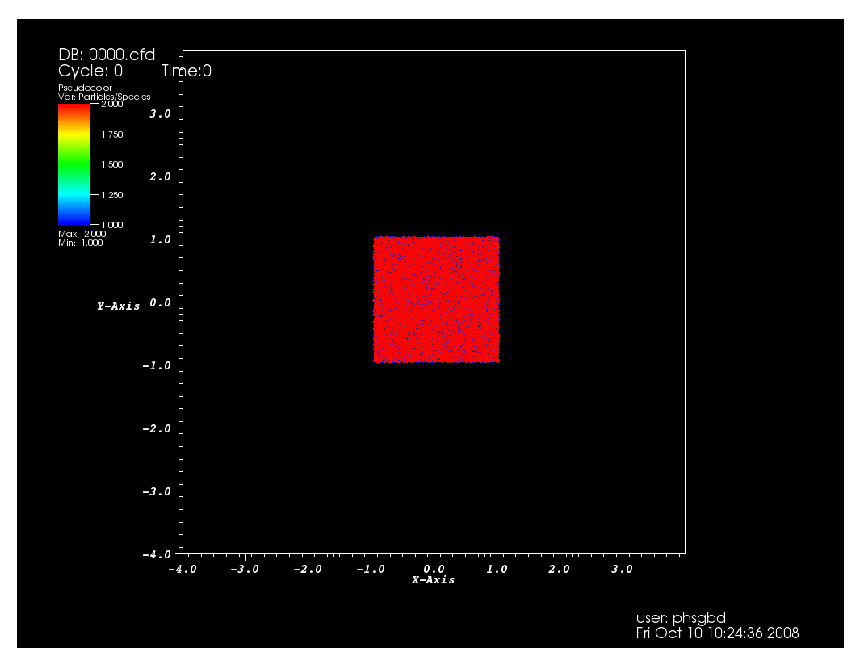
\includegraphics{./images/example3.eps}\\}
An important point to notice is that the two parts of the logical expressions in the input deck are enclosed within their own brackets. This helps to remove some ambiguities in the functioning of the input deck parser. It is hoped that this will soon be fixed, but at present ALWAYS enclose logical expressions in brackets.
\subsection{Deferred Evaluation Objects (DEOs)}
In addition to custom constants it is also possible to set up deferred execution objects. The difference between the two is that constants are immediatly evaluated when defined, so they cannot include the spatial information used in defining initial conditions. DEOs are evaluated at the point in the deck where they are used so they can include spatial information. DEOs are relativly memory intensive, so should only be used when required. An example would be
\begin{verbatim}
begin:deo
      r=sqrt(x^2+y^2)
end:deo

begin:species1
      #first set density in the range 0->1
      #cut down density in x direction
      rho=if ((r lt 1),1.0,0.2)


      #multiply density by real particle density
      rho=rho(1)*partdens

      #Set the temperature to be zero
      temp_x=0.0
      temp_y=temp_x(1)

      #Set the minimum density for this species
      minrho=0.3*partdens
end:species1
\end{verbatim}
This example produces a circular rather than a square density enhancement.

\subsection{Restarting EPOCH from previous output dumps}
Another possible way of setting up initial conditions in EPOCH is to load in a previous output dump and use it to specify initial conditions for the code. The effect of this is to restart the code from the state that it was in when the dump was made. To do this, you just specify ``initial\_conditions = restart'' in the input deck and then set the field ``restart\_snapshot'' to the number of the output dump from which you want the code to restart. Because of the way in which the code is written you cannot guarantee that the code can succesfully restart from any output dump. To restart properly, the following{\it must} have been dumped
\begin{itemize}
\item Particle positions
\item Particle momenta
\item Particle species
\item Particle weights
\item Relevant parts of the electric field (If for example it is known that Ez == 0 then it is not needed)
\item Relevant parts of the magnetic field
\end{itemize}
Since the autoloader completely changes the position of particles etc. it is not possible to combine restart dumps with {\it any} of the autoloader routines. It is possible to use the manual particle control part of the initial conditions to make changes to a restarted initial condition after the restart dump is loaded. The output files don't include all of the information needed to restart the code fully, so if you wish to archive output dumps for future use, you will need to retain a copy of all relevant input deck files with the output file as well. In future the code may well be changed to allow full restart from output files.\\

If specific ``restart'' dumps are specified in the input deck, or the ``force\_final\_to\_be\_restartable'' flag is set then in some cases the output is forced to contain enough information to output all the data. These restart dumps can be very large, and also override the ``dump'' parameter specified for a species and output the data for that species anyway.
\subsection{Visualising EPOCH output data}
\subsubsection{IDL}
EPOCH is supplied with routines to allow the visualisation of data from within the ITT IDL data analysis and visualisation language. To start IDL with the routines loaded, just type\\
\texttt{idl Start}\\
in the main EPOCH directory. To load an output, just type\\
\texttt{data=getdata(\{dumpnum\},datadir=''Data'')}\\
the return value from this function is an IDL structure which contains all the data which is available in the output dump. Some of the data which has been loaded is itself a structure because of the need to store some metadata as well as the primary data. For example particle position information in the x direction would be accessed using\\
\texttt{data.particles.particlepositions(*,0)}\\
in the y direction\\
\texttt{data.particles.particlepositions(*,1)}\\
etc. It is also possible to get more information about the data held in a given data dump by typing\\
\texttt{data=getdata(\{dumpnum\},datadir=''Data'',/variables)}\\
which prints the name and type of data held in the file, but loads no data. To load a specific variable, just add a /\{variable\_name\} to the load command\\
\texttt{data=getdata(\{dumpnum\},datadir=''Data'',/vx)}\\
\subsubsection{LLNL VisIT}
LLNL's VisIT software is a parallel data visualisation package(\texttt{https://wci.llnl.gov/codes/visit/}). EPOCH comes with source code for the plugin needed to allow VisIT to load the output CFD files which are generated. There are full manuals for VisIT which can be downloaded from the above link so no further details will be given here.
\subsubsection{Mathworks MatLab}
There are also routines to allow the loading of CFD files from Mathworks MatLab software. These are still under development so are not shipped with the code. If they are required, they can be supplied on demand.


\section{EPOCH for advanced end users}
\subsubsection{Setting autoloader parameters within EPOCH}
Within EPOCH, there are Fortran90 structures which represent the information needed by the autoloader for each species. In 2D, the definition of these structures is

\begin{verbatim}
  TYPE :: Initial_Condition_Block

     REAL(num),DIMENSION(:,:),ALLOCATABLE :: Rho !Number density
     REAL(num),DIMENSION(:,:,:),ALLOCATABLE :: Temp !Temperature
     REAL(num) :: minrho !Minimum density
     REAL(num) :: maxrho !Maximum density

  END TYPE Initial_Condition_Block
\end{verbatim}
In 1D, there is one fewer dimension to both arrays, and in 3D there is one more dimension to both arrays. An instance of the structure is created for each particle species and is named ``InitialConditions(iSpecies)''. The elements of this structure have the following definitions (again in 2D)\\
\begin{itemize}
\item Rho(-1:nx+2,-1:ny+2) - Particle {\bf NUMBER} density at all spatial positions in the grid. Must be defined fully between -1:nx+2 and -1:ny+2
\item Temp(-1:nx+2,-1:ny+2,1:3) - Temperature of a thermal distribution at all spatial positions in the grid, and independantly in each dimension (including ignorable directions). The final dimension is the direction in which to apply the specified thermal distribution.
\item minrho - The minimum density at which to load particles. If the initial particle number density at any point is lower then minrho then particles are not loaded there by the autoloader.
\item maxrho - The maximum density. If the initial particle number density exceeds maxrho then the density is clipped to maxrho.
\end{itemize}

So an example of setting up a cold plasma block for all species in 2D would look like
\begin{verbatim}
  SUBROUTINE IC_Early
     INTEGER :: iSpecies
     REAL(num) :: slab
     DO iSpecies=1,nSpecies
        InitialConditions(iSpecies)%Temp=0.0_num
        InitialConditions(iSpecies)%minrho=1.4_num
        DO iy=-1,ny+2
           DO ix=-1,nx+2
              slab=0.0_num
              IF (x(ix) .LT. 1.0_num .AND. x(ix) .GT. -1.0_num) slab=100.0
              InitialConditions(iSpecies)%Rho(ix,iy)=1.0_num + slab
           ENDDO
        ENDDO
     ENDDO
     
  END SUBROUTINE IC_Early
\end{verbatim}
This sets up a plasma slab with a density of 100 particles per square metre between x=-1 and x=+1 with no restriction on y. Note that density is never set to zero anywhere, the lowest value of rho is 1.0. However, since the minrho value is set to 1.4 then particles are only loaded inside the slab where the density is greater than 1.4. If rho had simply been set to zero (or worse, some small but non-zero number) the code would have positioned particles in that cell anyway, but would have assigned the particles very low or zero weight functions meaning that they would have barely contributed to the solution while at the same time taking up compute resources. If you have localised density slabs in a vacuum, you should always use the minrho parameter to set a cutoff below which particles are not loaded. Running this example gives the following (This picture was produced using LLNL visit to plot a subset of the particles. The apparantly ordered layout of particles is a result of the quiet start algorithm combined with the routine which selects a subset of the particles)\\
%Example image from visit for these initial conditions
{\center 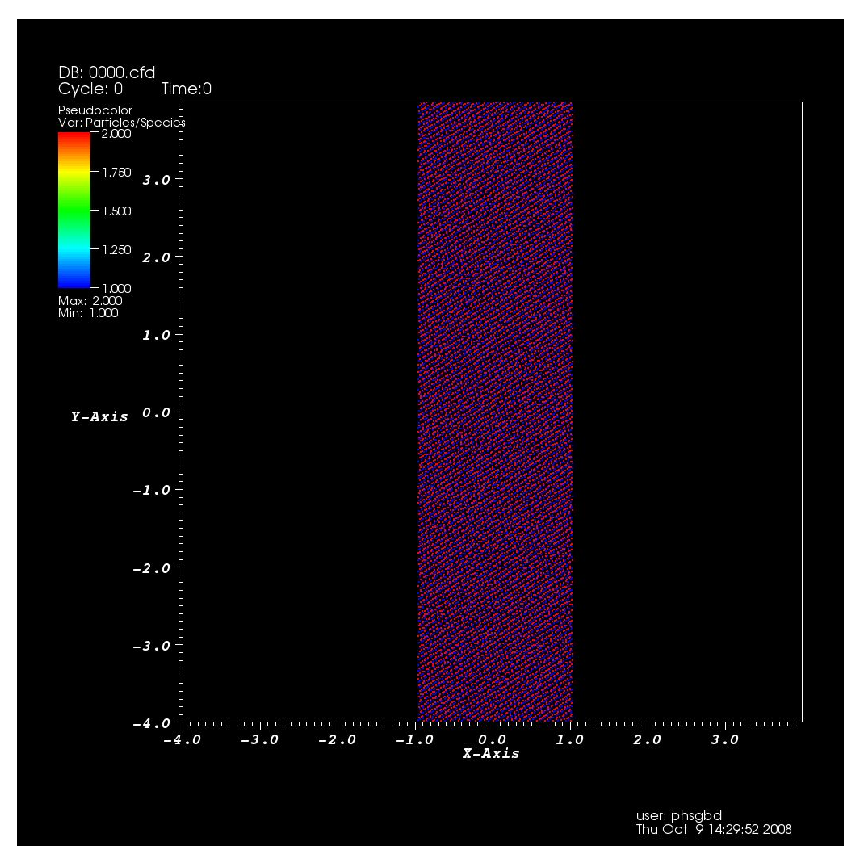
\includegraphics{./images/example.eps}\\}
In the given example the code is in the subroutine ``IC\_Early'', but since the external setup isn't used it could be copied freely into the ``IC\_Late'', only changing the input deck to tell EPOCH to use late internal initial conditions instead of early internal initial conditions. The only difference between the early and late internal initial conditions is that in ``IC\_Early'' the temperature and number density are guaranteed to be zero, whereas in ``IC\_Late'' they will contain any changes made in ``IC\_Early'' and in the external initial conditions. So to take a (very silly) example, I could use the following code to change the slab to have a finite width in y.

\begin{verbatim}
  SUBROUTINE IC_Late
     INTEGER :: iSpecies
     DO iSpecies=1,nSpecies
        DO iy=-1,ny+2
           DO ix=-1,nx+2
              IF (y(iy) .GT. 1.0_num .OR. y(iy) .LT. -1.0_num)&
                 InitialConditions(iSpecies)%Rho(ix,iy)=1.0_num
           ENDDO
        ENDDO
     ENDDO
     
  END SUBROUTINE IC_Late
\end{verbatim}
Once this has been added then changing ``initial\_conditions'' field of the input deck from ``initial\_conditions = internal\_early'' to ``initial\_conditions = internal\_early + internal\_late'' changes the output of the code from the previous figure to this one\\
%Example image from visit for the second set of initial conditions
{\center 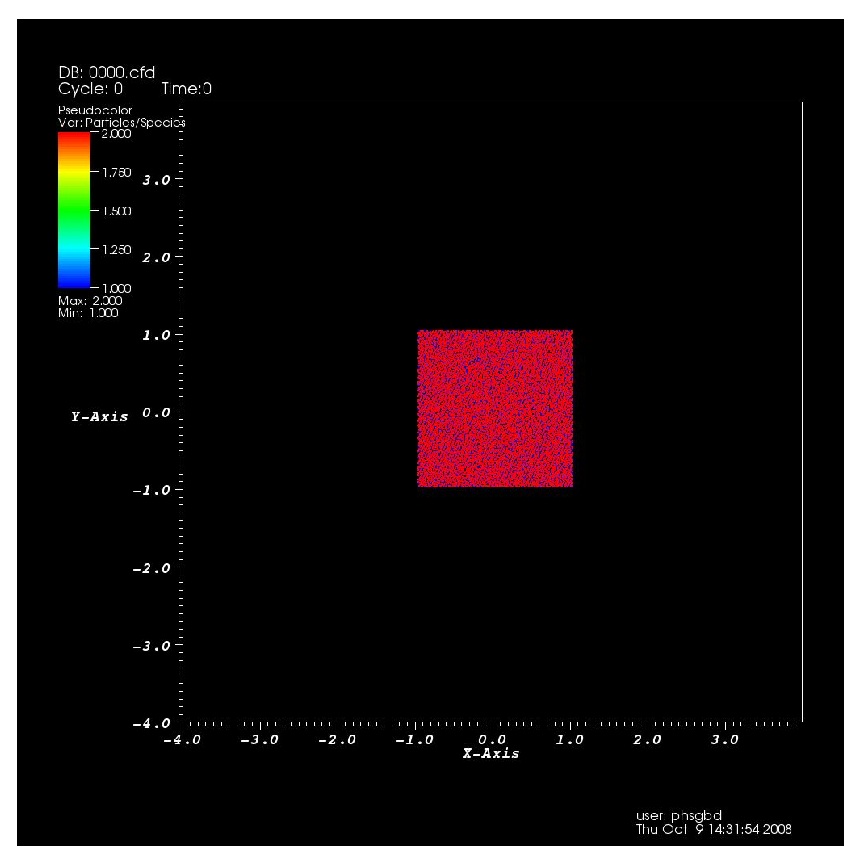
\includegraphics{./images/example2.eps}\\}
Both figures are from runs with the same number of particles and the same fraction of particles displayed in VisIT. This shows why the use of the minrho field is so useful, because the second figure obviously has a higher particles density than the first, since the particles are concentrated into a smaller region.
\end{document}
